\documentclass[12pt]{article}
\usepackage[a4paper,margin=2.5cm]{geometry}
\usepackage{amsmath, amssymb, amsthm}
\usepackage{bm}
\usepackage{hyperref}
\usepackage{graphicx}
\usepackage{caption}
\usepackage{listings}
\usepackage{xcolor}
\usepackage{float}
\usepackage{placeins}
\graphicspath{{figures/}}

% Code style
\lstdefinestyle{code}{
  basicstyle=\ttfamily\small,
  numbers=left,
  numberstyle=\tiny,
  numbersep=8pt,
  keywordstyle=\color{blue},
  commentstyle=\color{teal!70!black},
  stringstyle=\color{orange!70!black},
  showstringspaces=false,
  breaklines=true,
  frame=single,
  framerule=0.3pt,
  rulecolor=\color{black!15}
}
\lstset{style=code}

\title{Recurrent Neural Networks: Theory and Practice}
\author{}
\date{\today}

\begin{document}
\maketitle

\section{RNN Structure and Core Principles}
Recurrent neural networks (RNNs) process sequential data by maintaining a hidden state $\mathbf{h}_t$ that aggregates past information. A simple Elman RNN updates
\begin{align}
  \mathbf{a}_t &= \mathbf{W}_{xh} \mathbf{x}_t + \mathbf{W}_{hh} \mathbf{h}_{t-1} + \mathbf{b}_h, \\
  \mathbf{h}_t &= \phi(\mathbf{a}_t), \\
  \mathbf{y}_t &= \mathbf{W}_{hy} \mathbf{h}_t + \mathbf{b}_y,
\end{align}
where $\phi$ is typically $\tanh$ or ReLU. Figure~\ref{fig:rnn_unrolled} depicts the recurrent computation graph unrolled in time.

\subsection{Unrolling and Backpropagation Through Time}
Training involves unfolding the network over $T$ steps and applying backpropagation through time (BPTT). Gradients of the loss $\mathcal{L}$ with respect to parameters accumulate contributions from each timestep:
\begin{equation}
  \frac{\partial \mathcal{L}}{\partial \mathbf{W}_{hh}} = \sum_{t=1}^{T} \left( \frac{\partial \mathcal{L}}{\partial \mathbf{a}_t} \frac{\partial \mathbf{a}_t}{\partial \mathbf{W}_{hh}} \right).
\end{equation}
Repeated multiplication by $\mathbf{W}_{hh}$ can cause exploding or vanishing gradients. Gradient clipping and orthogonal initialization mitigate instability.

\subsection{Variants of Recurrent Connections}
Bidirectional RNNs process sequences in both forward and backward directions, concatenating hidden states to capture past and future context. Deep (stacked) RNNs add layers of recurrence for hierarchical representations. Residual and highway connections ease optimization by facilitating gradient flow across layers.

\begin{lstlisting}[language=Python, caption={PyTorch Elman RNN cell with gated recurrent unit interface.}]
import torch
import torch.nn as nn

class SimpleRNNCell(nn.Module):
    def __init__(self, input_size, hidden_size):
        super().__init__()
        self.Wxh = nn.Linear(input_size, hidden_size)
        self.Whh = nn.Linear(hidden_size, hidden_size)

    def forward(self, x_t, h_prev):
        a_t = self.Wxh(x_t) + self.Whh(h_prev)
        h_t = torch.tanh(a_t)
        return h_t
\end{lstlisting}

\begin{figure}[H]
  \centering
  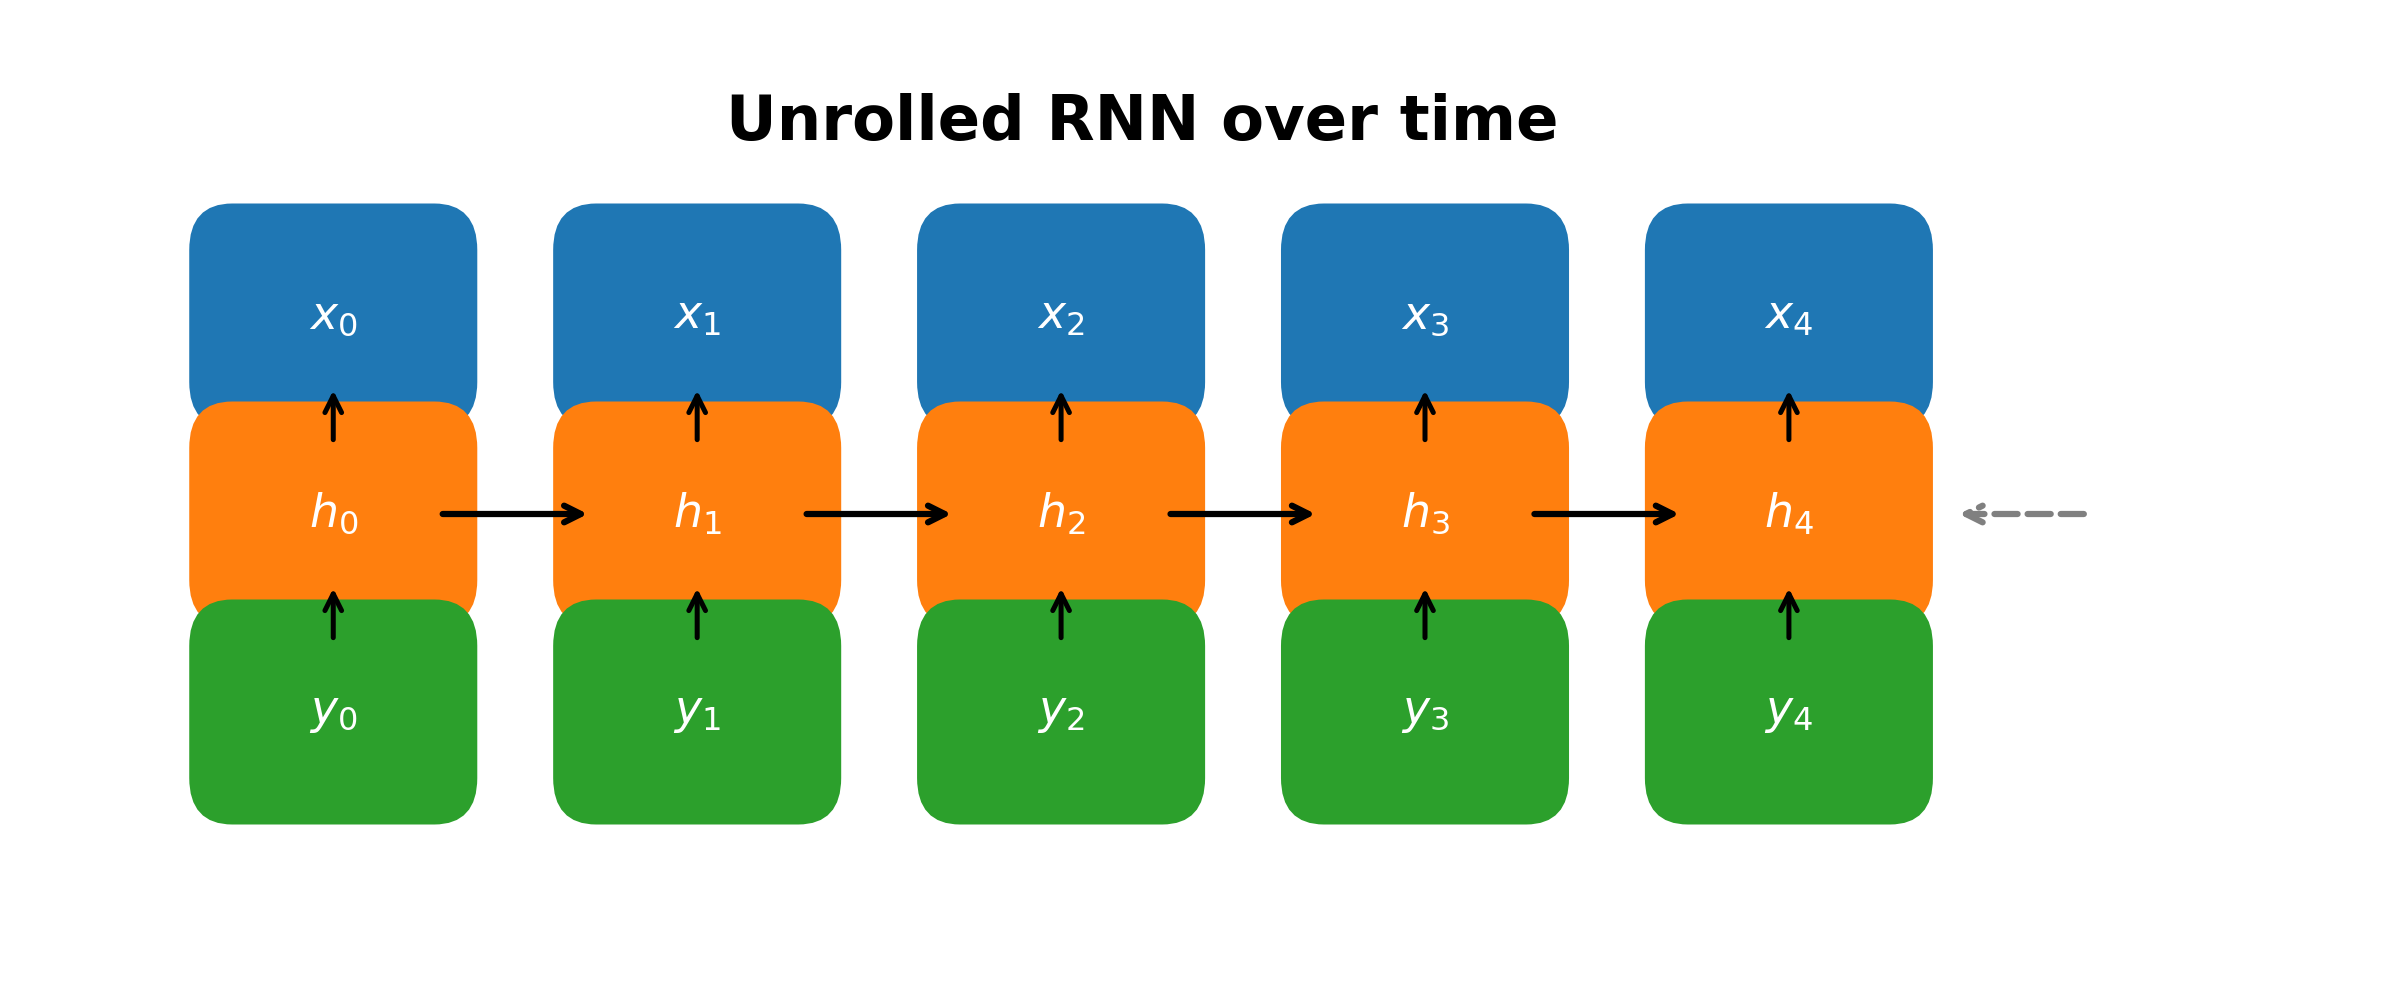
\includegraphics[width=0.85\linewidth]{rnn_unrolled_dynamics.png}
  \caption{Unrolled recurrent computation showing information flow and hidden-to-hidden transitions.}
  \label{fig:rnn_unrolled}
\end{figure}
\FloatBarrier

\section{LSTM and GRU Architectures}
Long short-term memory (LSTM) and gated recurrent units (GRU) introduce gating mechanisms to alleviate vanishing gradients and capture long-range dependencies. Figure~\ref{fig:lstm_gru} compares their gates.

\subsection{LSTM Structure}
An LSTM cell maintains a cell state $\mathbf{c}_t$ alongside the hidden state $\mathbf{h}_t$. Gates regulate information flow:
\begin{align}
  \mathbf{f}_t &= \sigma(\mathbf{W}_f [\mathbf{x}_t, \mathbf{h}_{t-1}] + \mathbf{b}_f), \\
  \mathbf{i}_t &= \sigma(\mathbf{W}_i [\mathbf{x}_t, \mathbf{h}_{t-1}] + \mathbf{b}_i), \\
  \tilde{\mathbf{c}}_t &= \tanh(\mathbf{W}_c [\mathbf{x}_t, \mathbf{h}_{t-1}] + \mathbf{b}_c), \\
  \mathbf{c}_t &= \mathbf{f}_t \odot \mathbf{c}_{t-1} + \mathbf{i}_t \odot \tilde{\mathbf{c}}_t, \\
  \mathbf{o}_t &= \sigma(\mathbf{W}_o [\mathbf{x}_t, \mathbf{h}_{t-1}] + \mathbf{b}_o), \\
  \mathbf{h}_t &= \mathbf{o}_t \odot \tanh(\mathbf{c}_t).
\end{align}
The forget gate $\mathbf{f}_t$ preserves long-term context, while input and output gates control updates and exposure.

\subsection{GRU Structure}
GRUs simplify LSTMs by combining cell and hidden states. Update and reset gates compute
\begin{align}
  \mathbf{z}_t &= \sigma(\mathbf{W}_z [\mathbf{x}_t, \mathbf{h}_{t-1}] + \mathbf{b}_z), \\
  \mathbf{r}_t &= \sigma(\mathbf{W}_r [\mathbf{x}_t, \mathbf{h}_{t-1}] + \mathbf{b}_r), \\
  \tilde{\mathbf{h}}_t &= \tanh(\mathbf{W}_h [\mathbf{x}_t, \mathbf{r}_t \odot \mathbf{h}_{t-1}] + \mathbf{b}_h), \\
  \mathbf{h}_t &= (1 - \mathbf{z}_t) \odot \mathbf{h}_{t-1} + \mathbf{z}_t \odot \tilde{\mathbf{h}}_t.
\end{align}
GRUs require fewer parameters and often converge faster while retaining the ability to model dependencies.

\subsection{Gate Dynamics}
LSTMs and GRUs both rely on sigmoid gates to scale prior states. Peephole connections allow gates to observe the cell state directly. Layer normalization within gates stabilizes training for long sequences.

\begin{figure}[H]
  \centering
  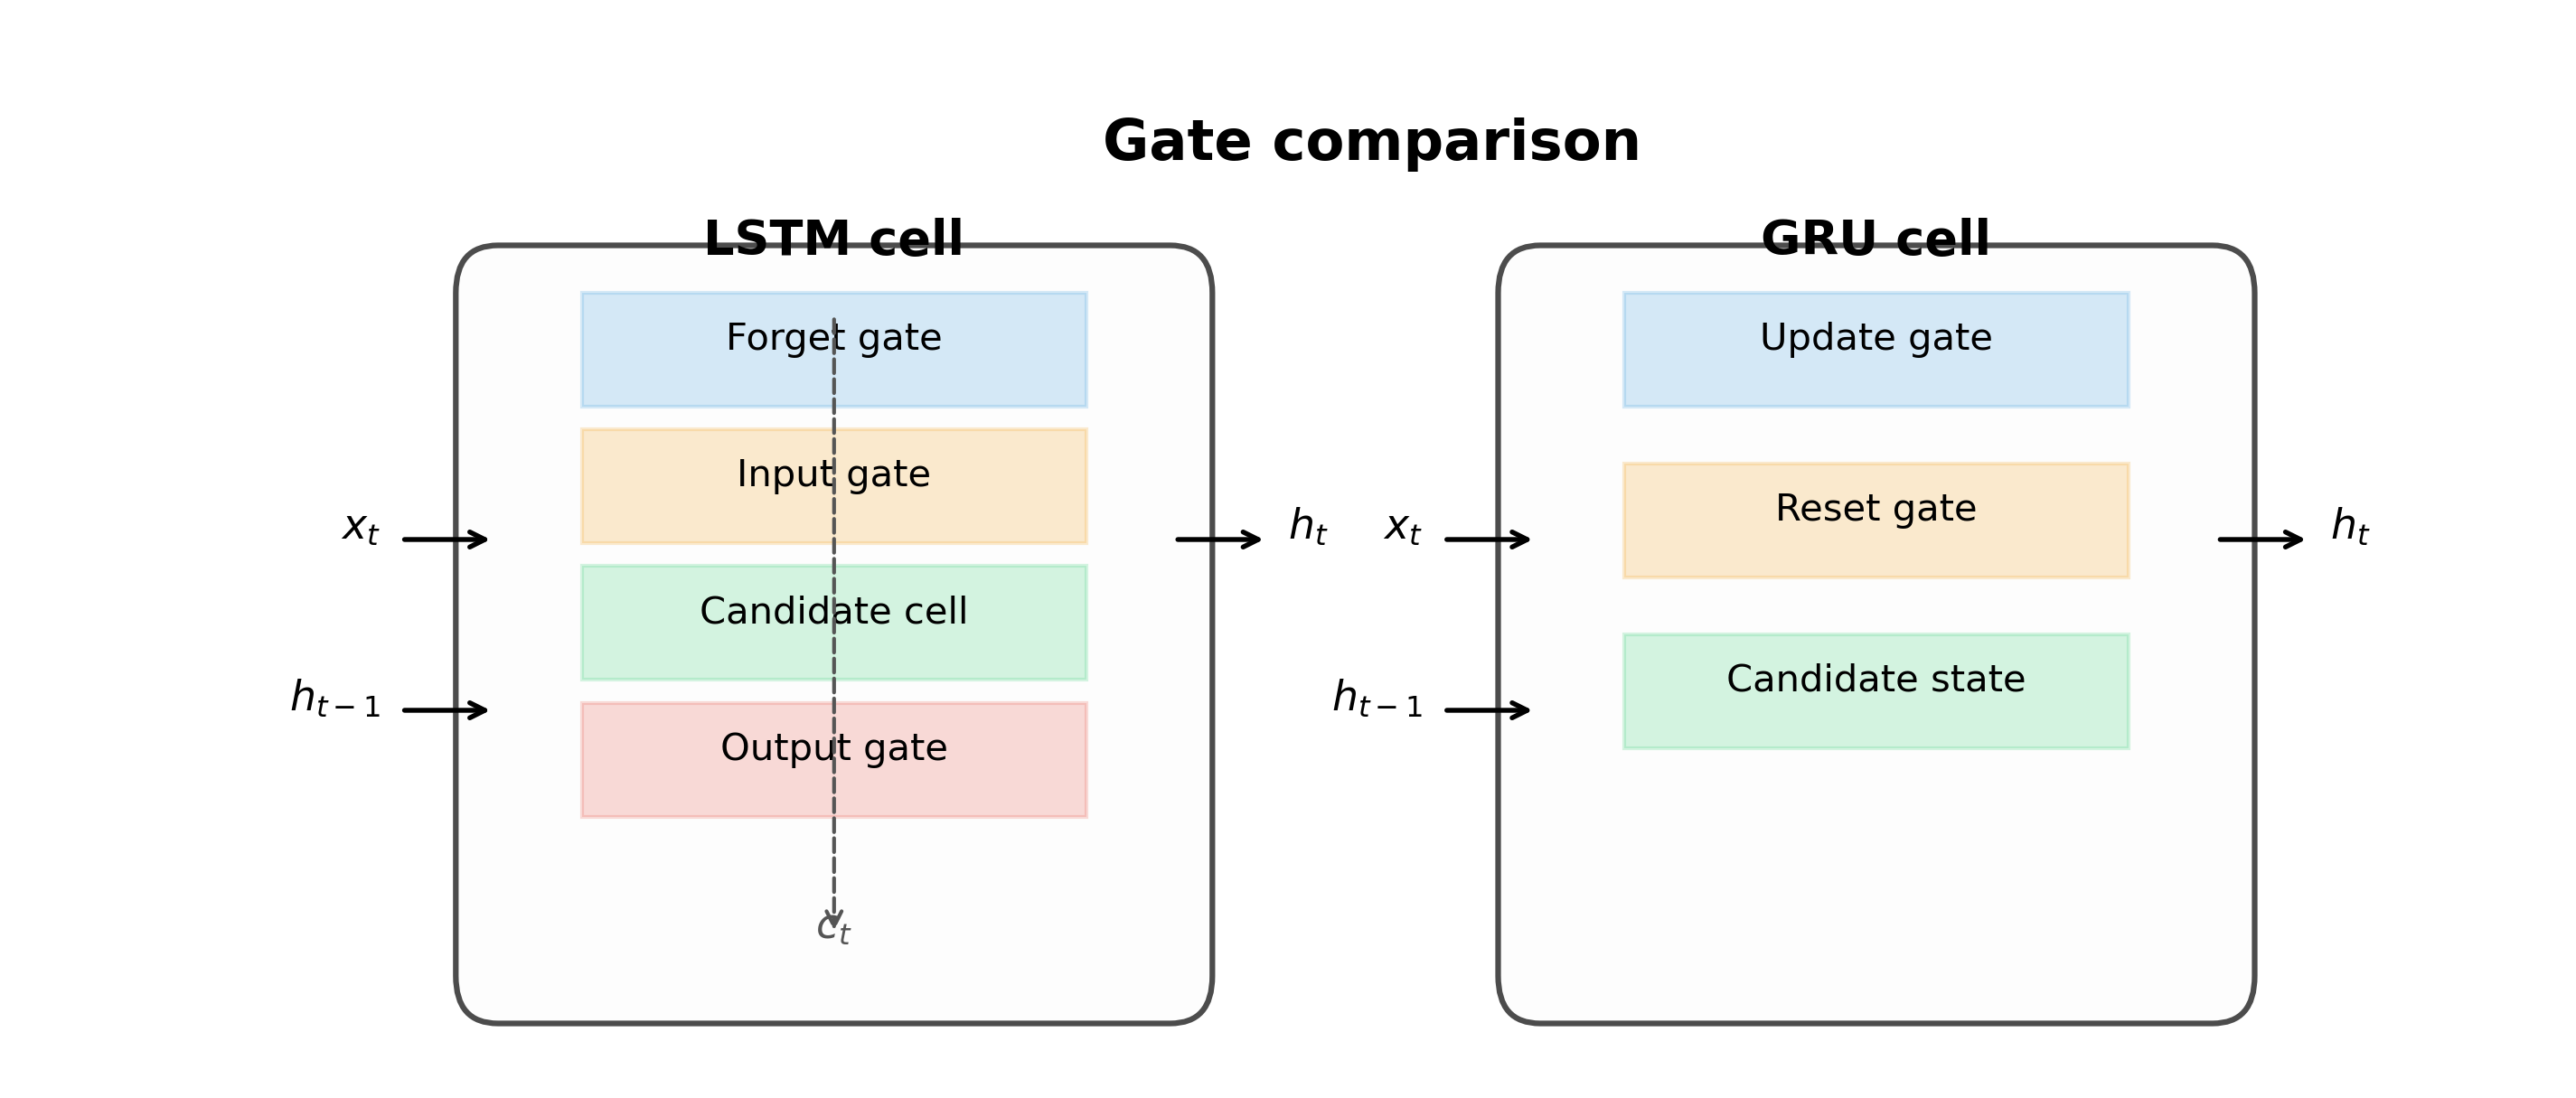
\includegraphics[width=0.85\linewidth]{lstm_gru_gate_comparison.png}
  \caption{Gating structures of LSTM and GRU cells highlighting information flow.}
  \label{fig:lstm_gru}
\end{figure}
\FloatBarrier

\section{Applications of RNNs}
RNNs excel at modeling temporal and sequential data across domains. Figure~\ref{fig:rnn_applications} outlines representative pipelines.

\subsection{Time-Series Forecasting}
For forecasting, RNNs ingest historical measurements to predict future values. Encoder-decoder architectures with attention capture long-range dependencies. Probabilistic outputs (Gaussian mixtures, quantile losses) quantify uncertainty.

\subsection{Text Generation and Language Modeling}
Character- or word-level RNNs model conditional distributions $p(w_t \mid w_{<t})$. Techniques such as teacher forcing, scheduled sampling, and temperature sampling influence generation quality. Combining RNNs with embeddings and subword tokenization improves representation.

\subsection{Speech and Audio Modeling}
RNNs represent variable-length acoustic sequences for speech recognition or synthesis. Connectionist temporal classification (CTC) aligns RNN outputs to transcriptions without frame-level labels. In text-to-speech, autoregressive vocoders (e.g., WaveRNN) generate waveforms sample by sample.

\subsection{Hybrid Architectures}
Attention mechanisms and transformers build on RNNs by reweighting sequence elements. Neural ordinary differential equations (Neural ODE) and continuous-time RNNs model irregularly sampled data. Lightweight gated RNNs (SRU, QRNN) reduce sequential dependencies for faster inference.

\begin{figure}[H]
  \centering
  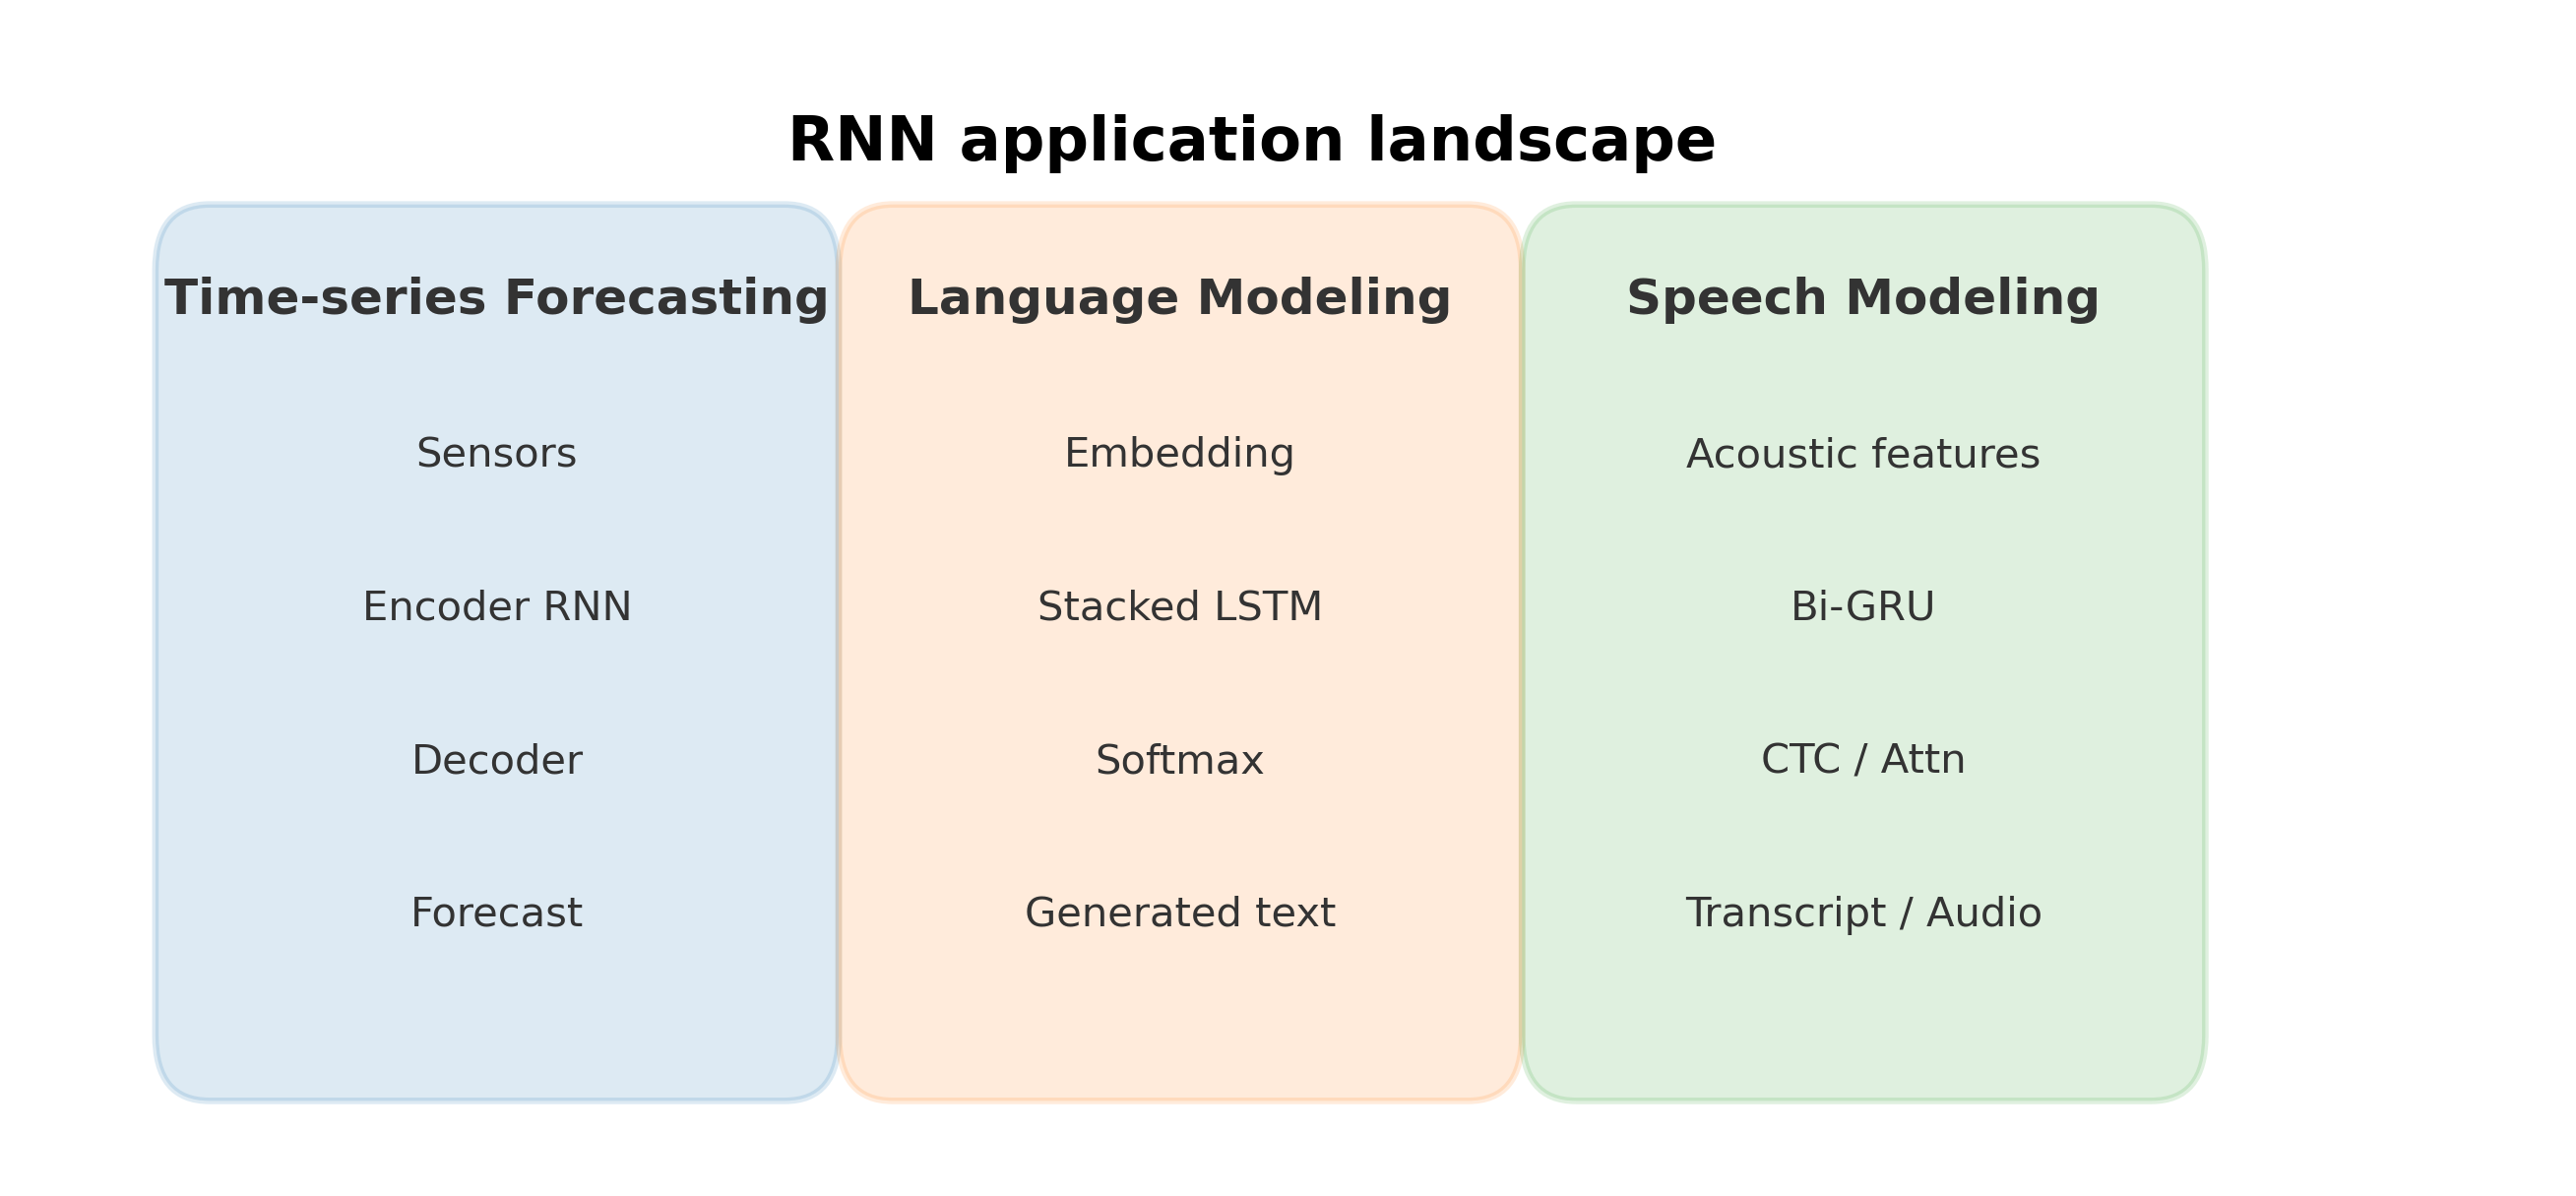
\includegraphics[width=0.85\linewidth]{rnn_applications_overview.png}
  \caption{RNN application pipelines: forecasting, language modeling, and speech processing.}
  \label{fig:rnn_applications}
\end{figure}
\FloatBarrier

\section{Practical Considerations}
\begin{itemize}
  \item \textbf{Sequence length:} Truncated BPTT balances context coverage and computational cost.\item \textbf{Regularization:} Apply dropout on inputs, recurrent dropout (variational dropout), or weight decay to prevent overfitting.\item \textbf{Initialization:} Orthogonal initialization for recurrent matrices preserves gradient norms.\item \textbf{Optimization:} Momentum SGD or Adam with gradient clipping (e.g., global norm) stabilizes training.\item \textbf{Monitoring:} Track perplexity for language models, mean absolute error for forecasting, and character error rate (CER) for speech tasks.\end{itemize}

\end{document}
